\documentclass[12pt,a4paper]{article}
\usepackage[utf8]{inputenc}
\usepackage[spanish, provide=*]{babel}
\usepackage[T1]{fontenc}
\usepackage{lmodern}
\usepackage{geometry}
\geometry{top=2cm, bottom=2cm, left=2.5cm, right=2.5cm}
\usepackage{xcolor}
\usepackage{listings}
\usepackage{enumitem}
\usepackage{fancyhdr}
\usepackage{hyperref}
\usepackage{tikz}
\usetikzlibrary{arrows.meta, positioning, calc, shapes.geometric}

\definecolor{codegreen}{rgb}{0,0.6,0}
\definecolor{backcolour}{rgb}{0.95,0.95,0.92}

\lstset{
    language=C,
    backgroundcolor=\color{backcolour},
    commentstyle=\color{codegreen},
    keywordstyle=\color{blue},
    basicstyle=\ttfamily\small,
    breaklines=true,
    frame=single,
    numbers=left,
    tabsize=4,
    extendedchars=true,
    showstringspaces=false,
    literate={á}{{\'a}}1 {é}{{\'e}}1 {í}{{\'i}}1 {ó}{{\'o}}1 {ú}{{\'u}}1 {ñ}{{\~n}}1
}

\pagestyle{fancy}
\fancyhf{}
\lhead{Monitorías Sistemas Operativos 2026-I}
\rhead{Examen: Pre-Parcial 2}
\cfoot{\thepage}

\title{\textbf{Examen Pre-Parcial 2: Simulador de Red Eléctrica Inteligente}}
\author{Malak Sanchez \\ \small Monitorías de Sistemas Operativos}
\date{\today}

\begin{document}

\maketitle

\section*{Introducción}
Este pre-parcial evalúa el diseño y la implementación de una arquitectura de procesamiento concurrente mediante hilos POSIX (\texttt{pthreads}). Deberá procesar grandes volúmenes de datos utilizando una técnica de \textbf{lotes (batches)} para limitar el uso de memoria, coordinando el flujo continuo de entrada/salida y procesamiento en paralelo empleando mecanismos de sincronización de barreras y exclusión mutua.

\section*{\textbf{Procesamiento por Lotes y Smart Grid}}

Usted debe construir un simulador que diagnostique el consumo eléctrico de múltiples zonas. Los datos históricos se proveen de manera secuencial a través de un archivo de texto. Para simular el entorno de baja memoria, se ha prohibido cargar la totalidad del archivo en un solo instante; el procesamiento debe limitarse a una lectura en bloques de tamaño $B$.

El sistema es administrado por el \textbf{Hilo Principal} y procesado cooperativamente por $H$ \textbf{Hilos Trabajadores (Analistas)}.

\subsection*{Estructura de Fases}
El programa iterará hasta procesar todos los elementos, dividido en las siguientes etapas operativas:

\begin{enumerate}
    \item \textbf{Fase 1 (I/O Sequencial):} El hilo principal lee un máximo de $B$ registros de consumo desde el archivo y los almacena en un arreglo global. Los hilos trabajadores deben esperar inactivos hasta que el hilo principal haya cargado completamente la información.
    
    \item \textbf{Fase 2 (Análisis Local Paralelo):} Una vez finalizada la carga, el hilo principal y todos los trabajadores rompen la Fase. Los $H$ hilos se reparten la tarea de evaluar el lote actual de consumos de forma equitativa. 
    Si la zona específica que evalúa registra un consumo \textbf{mayor a 150 MW}, el hilo \textbf{incrementará un contador global de Alertas Locales}.
    
    \item \textbf{Fase 3 (Análisis Global):} Al mismo tiempo, el Hilo Principal tomará el arreglo del lote y realizará una sumatoria de los $B$ elementos para obtener el \textbf{Consumo Total del Lote}. Si este consumo acumulado del lote excede el límite crítico global ($C = B \times 130$ MW), el Hilo Principal \textbf{incrementará un contador global de Apagones}.
    
    \item \textbf{Finaización (Sincronización):} Todo el equipo requiere re-agruparse. El Hilo Principal \textbf{no puede sobreescribir} y cargar el siguiente lote del archivo si algún trabajador todavía se encuentra analizando datos del lote actual.
\end{enumerate}

Para esto, se debe utilizar obligatoriamente exclusión mutua sobre los contadores globales que presenten una potencial \textbf{condición de carrera}.

\newpage

\section*{Formato de Entrada y Salida}
El programa será invocado como \texttt{./smartgrid <archivo> <H>}, donde $H$ es el total de hilos analistas. 
La primera línea del archivo dicta la cantidad total $N$ de datos y el tamaño máximo $B$ de elementos a cargar por corrida \textit{(Batch Size)}.

\vspace{0.4cm}
\noindent
\begin{minipage}[t]{0.48\textwidth}
\textbf{Ejemplo de archivo (\texttt{consumos.txt})}
\begin{lstlisting}[numbers=none, frame=single, backgroundcolor=\color{white}]
12 4
120
160
180
100
170
95
195
190
130
140
160
110
\end{lstlisting}
\vspace{0.1cm}
\textit{*(12 consumos totales, cargados de 4 en 4)*}
\end{minipage}
\hfill
\begin{minipage}[t]{0.48\textwidth}
\textbf{Salida Esperada (Intercalada)}
\begin{lstlisting}[numbers=none, frame=single, backgroundcolor=\color{white}]
[Lote 1] Alerta: Zona en Riesgo. 160 MW
[Lote 1] Alerta: Zona en Riesgo. 180 MW
[Lote 1] Alerta Global de Apagon. 560 MW.
...
----- REPORTE FINAL -----
Total Alertas Locales procesadas: X
Total Alertas Globales (Apagones): Y
Todos los recursos finalizados exitosamente.
\end{lstlisting}
\end{minipage}

\vspace{0.8cm}
\begin{center}
\makebox[\textwidth][c]{
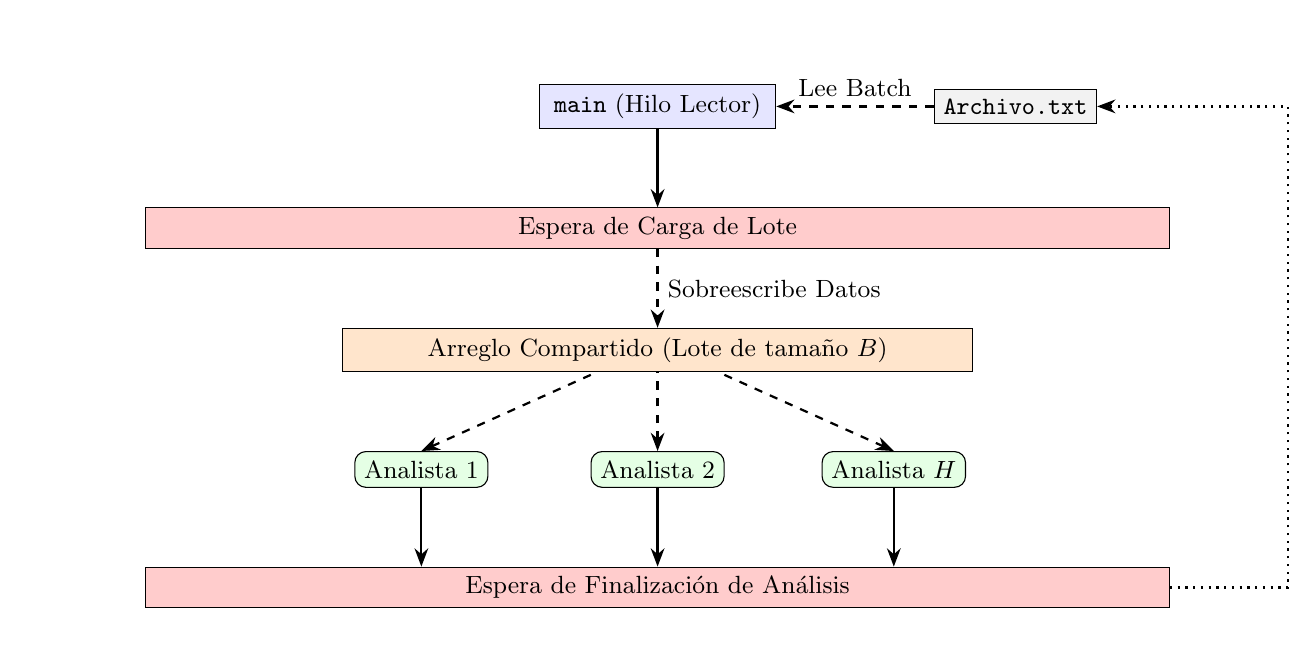
\begin{tikzpicture}[node distance=1.5cm, font=\small, >=Stealth]
    \useasboundingbox (-8,-6.5) rectangle (8,1);
    \node[draw, rectangle, fill=blue!10, minimum width=3cm] (master) {\texttt{main} (Hilo Lector)};
    \node[draw, rectangle, fill=gray!10, right=2cm of master] (file) {\texttt{Archivo.txt}};
    
    \node[draw, rectangle, fill=red!20, below=1cm of master, minimum width=13cm] (b1) {Espera de Carga de Lote};
    
    \node[draw, rectangle, fill=orange!20, below=1cm of b1, minimum width=8cm] (data) {Arreglo Compartido (Lote de tamaño $B$)};
    
    \node[draw, rounded corners, fill=green!10, below=1cm of data, xshift=-3cm] (h1) {Analista 1};
    \node[draw, rounded corners, fill=green!10, below=1cm of data, xshift=0cm] (h2) {Analista 2};
    \node[draw, rounded corners, fill=green!10, below=1cm of data, xshift=3cm] (h3) {Analista $H$};
    
    \node[draw, rectangle, fill=red!20, below=1cm of h2, minimum width=13cm] (b2) {Espera de Finalización de Análisis};

    \draw[->, thick, dashed] (file.west) -- (master.east) node[midway, above] {Lee Batch};
    
    \draw[->, thick] (master.south) -- (b1.north);
    \draw[->, thick, dashed] (b1.south) -- (data.north) node[midway, right] {Sobreescribe Datos};
    
    \draw[<-, thick, dashed] (h1.north) -- (data.200);
    \draw[<-, thick, dashed] (h2.north) -- (data.270);
    \draw[<-, thick, dashed] (h3.north) -- (data.340);
    
    \draw[->, thick] (h1.south) -- (b2.north -| h1);
    \draw[->, thick] (h2.south) -- (b2.north);
    \draw[->, thick] (h3.south) -- (b2.north -| h3);
    
    \draw[->, thick, dotted] (b2.east) -- +(1.5cm,0) |- (file.east);
\end{tikzpicture}
}
\end{center}

\newpage

\section*{Requerimientos Técnicos y Reglas}
\begin{itemize}[itemsep=1ex]
    \item Todo acceso para incrementar o modificar las dos variables globales de acumulación final debe ser defendido bajo previas llamadas de adquisición de exclusión mutua propiamente dicha.
    \item El mecanismo utilizado para coordinar la lectura secuencial seguida de paralela iterativamente requiere instanciar estrictamente mecanismos de bloqueo tipo barrera. Estos deben esperar a que se presenten todos los hilos, contando el $H$ de trabajadores y $\mathbf{1}$ hilo principal.
    \item Los hilos trabajadores deben finalizar sus rutinas elegantemente y retornar mediante \texttt{pthread\_join} una vez se agote el procesamiento del archivo.
\end{itemize}

\end{document}
